\documentclass[11pt,a4paper]{article}
\usepackage[utf8]{inputenc}
\usepackage[margin=1.5cm]{geometry}
\usepackage{amsmath,amssymb,amsfonts}
\usepackage{xcolor}
\usepackage{graphicx}
\usepackage{booktabs}
\usepackage{array}
\usepackage{caption}
\usepackage{subcaption}

% TikZ & Libraries
\usepackage{tikz}
\usetikzlibrary{
    arrows.meta,
    positioning,
    calc,
    shapes.geometric,
    shapes.misc,
    backgrounds,
    fit,
    matrix,
    decorations.pathreplacing,
    shadows.blur,
    patterns
}

% ==============================================================================
% COLOR PALETTE (Modern Scientific / IEEE / CVPR Publication Standard)
% ==============================================================================
% Visual Branch Palette
\definecolor{visHeader}{RGB}{24, 76, 120}
\definecolor{visBg}{RGB}{246, 250, 255}
\definecolor{clipBorder}{RGB}{41, 128, 185}
\definecolor{clipFill}{RGB}{232, 242, 254}
\definecolor{clipText}{RGB}{18, 65, 105}

% EAA (Face Adapter) Palette
\definecolor{eaaBorder}{RGB}{39, 174, 96}
\definecolor{eaaFill}{RGB}{235, 251, 241}
\definecolor{eaaText}{RGB}{20, 90, 50}

% CMAF Fusion Palette
\definecolor{cmafBorder}{RGB}{230, 126, 34}
\definecolor{cmafFill}{RGB}{254, 246, 237}
\definecolor{cmafText}{RGB}{125, 60, 15}

% Temporal & Pooling Palette
\definecolor{tempBorder}{RGB}{142, 68, 173}
\definecolor{tempFill}{RGB}{247, 240, 252}
\definecolor{tempText}{RGB}{81, 35, 102}

\definecolor{poolBorder}{RGB}{214, 51, 132}
\definecolor{poolFill}{RGB}{253, 239, 247}
\definecolor{poolText}{RGB}{120, 20, 70}

% Text Branch Palette
\definecolor{textHeader}{RGB}{30, 130, 76}
\definecolor{textBg}{RGB}{245, 253, 247}
\definecolor{promptBorder}{RGB}{22, 160, 133}
\definecolor{promptFill}{RGB}{230, 249, 245}
\definecolor{descBorder}{RGB}{108, 92, 231}
\definecolor{descFill}{RGB}{243, 240, 253}

% Losses & Projections
\definecolor{lossBorder}{RGB}{231, 76, 60}
\definecolor{lossFill}{RGB}{253, 237, 236}
\definecolor{lossText}{RGB}{146, 43, 33}

\definecolor{midcBorder}{RGB}{243, 156, 18}
\definecolor{midcFill}{RGB}{254, 249, 231}

\definecolor{vecBorder}{RGB}{211, 84, 0}
\definecolor{vecFill}{RGB}{253, 235, 220}

\definecolor{grayBorder}{RGB}{127, 140, 141}
\definecolor{grayFill}{RGB}{242, 244, 244}

% ==============================================================================
% TIKZ STYLES DEFINITION
% ==============================================================================
\tikzset{
    >={Latex[length=2.4mm, width=1.8mm]},
    baseNode/.style={
        rectangle,
        rounded corners=3.5pt,
        align=center,
        inner sep=4pt,
        font=\footnotesize,
        line width=0.8pt,
        blur shadow={shadow blur steps=3, shadow blur radius=1.5pt, opacity=0.15}
    },
    inputNode/.style={
        baseNode,
        draw=grayBorder,
        fill=white,
        font=\scriptsize,
        minimum height=1.6cm,
        minimum width=1.4cm
    },
    clipNode/.style={
        baseNode,
        draw=clipBorder,
        fill=clipFill,
        text=clipText,
        minimum width=2.4cm,
        minimum height=1.1cm
    },
    eaaNode/.style={
        baseNode,
        draw=eaaBorder,
        fill=eaaFill,
        text=eaaText,
        minimum width=2.3cm,
        minimum height=1.1cm
    },
    cmafNode/.style={
        baseNode,
        draw=cmafBorder,
        fill=cmafFill,
        text=cmafText,
        minimum width=2.5cm,
        minimum height=2.8cm
    },
    tempNode/.style={
        baseNode,
        draw=tempBorder,
        fill=tempFill,
        text=tempText,
        minimum width=2.4cm,
        minimum height=1.1cm
    },
    poolNode/.style={
        baseNode,
        draw=poolBorder,
        fill=poolFill,
        text=poolText,
        minimum width=1.7cm,
        minimum height=1.1cm
    },
    projNode/.style={
        baseNode,
        draw=grayBorder,
        fill=grayFill,
        text=black!80,
        minimum width=1.2cm,
        minimum height=1.1cm
    },
    vecNode/.style={
        circle,
        draw=vecBorder,
        fill=vecFill,
        text=vecBorder!90!black,
        inner sep=1.5pt,
        font=\scriptsize\bfseries,
        line width=0.9pt
    },
    lossNode/.style={
        baseNode,
        draw=lossBorder,
        fill=lossFill,
        text=lossText,
        font=\scriptsize\bfseries,
        minimum width=1.8cm,
        minimum height=1.1cm
    },
    textNode/.style={
        baseNode,
        draw=promptBorder,
        fill=promptFill,
        text=promptBorder!90!black,
        minimum width=2.4cm,
        minimum height=1.0cm
    },
    descNode/.style={
        baseNode,
        draw=descBorder,
        fill=descFill,
        text=descBorder!90!black,
        minimum width=2.4cm,
        minimum height=1.0cm
    },
    midcNode/.style={
        baseNode,
        draw=midcBorder,
        fill=midcFill,
        text=midcBorder!90!black,
        minimum width=2.0cm,
        minimum height=1.8cm
    },
    dimLabel/.style={
        font=\tiny\ttfamily,
        text=black!60,
        inner sep=1pt
    },
    mathLabel/.style={
        font=\scriptsize,
        text=black!75
    },
    flowArrow/.style={
        ->,
        line width=0.85pt,
        draw=black!75
    },
    lossArrow/.style={
        ->,
        line width=0.9pt,
        draw=lossBorder,
        dashed
    },
    sharedLine/.style={
        draw=black!40,
        dashed,
        line width=0.7pt
    }
}

\title{\Large\bfseries Detailed Architecture Diagram of RAPT-CLIP\\
\large Frame-Level Cross-Modal Attention Fusion for Video Emotion Recognition}
\author{\textbf{Research Technical Documentation \& Manuscript Vector Specification}}
\date{\today}

\begin{document}

\maketitle

\section*{Overview of Architectural Components \& Tensor Dimensions}
This document specifies the exact tensor flow, architectural modules, and mathematical objectives of the \textbf{RAPT-CLIP} framework. The architecture addresses extreme class imbalance and micro-expression subtlety in video classroom emotion recognition (RAER, DAiSEE, CAER-S).

\begin{table}[h!]
\centering
\small
\renewcommand{\arraystretch}{1.2}
\begin{tabular}{@{}llll@{}}
\toprule
\textbf{Module} & \textbf{Input Tensor Shape} & \textbf{Output Tensor Shape} & \textbf{Key Operations / Parameters} \\
\midrule
\textbf{Video Stream Inputs} & $V \in \mathbb{R}^{B \times T \times 3 \times H \times W}$ & $F_{1..T}, B_{1..T}, C_{1..T} \in \mathbb{R}^{B \times T \times 3 \times 224 \times 224}$ & Cropping: Face (MTCNN), Body, Context ($T=16$) \\
\textbf{Visual Backbone} & $\mathbb{R}^{(B \cdot T) \times 3 \times 224 \times 224}$ & $\mathbf{z}_t \in \mathbb{R}^{(B \cdot T) \times 512}$ & CLIP ViT-B/16 (Shared weights, 12 layers, 196 patches) \\
\textbf{Face Adapter (EAA)} & $\mathbf{z}_t^{\text{face}} \in \mathbb{R}^{(B \cdot T) \times 512}$ & $\mathbf{f}_t^{\text{face}} \in \mathbb{R}^{(B \cdot T) \times 512}$ & Bottleneck: $512 \!\rightarrow\! 128 \!\rightarrow\! 512$, ReLU, Drop($0.5$), Residual, Drop($0.3$) \\
\textbf{CMAF Frame Fusion} & $3 \times \mathbb{R}^{(B \cdot T) \times 512}$ & $\mathbf{f}_t \in \mathbb{R}^{(B \cdot T) \times 1536}$ (or $1024$) & Tridirectional Multi-Head Cross Attention ($h=4$) + Concat \\
\textbf{Temporal Transformer} & $\mathbf{f}_{1..T} \in \mathbb{R}^{B \times 16 \times 1536}$ & $\mathbf{H} \in \mathbb{R}^{B \times 16 \times 1536}$ & 1 Layer, $h=8$, Positional Embedding, Pre-LN, FFN(1024) \\
\textbf{Attention Pooling} & $\mathbf{H} \in \mathbb{R}^{B \times 16 \times 1536}$ & $\mathbf{F} \in \mathbb{R}^{B \times 1536}$ & $\alpha_t = \text{Softmax}(\mathbf{w}_2^\top \tanh(\mathbf{W}_1 \mathbf{h}_t + \mathbf{b}_1))$, $\mathbf{F} = \sum_{t} \alpha_t \mathbf{h}_t$ \\
\textbf{Projection \& Norm} & $\mathbf{F} \in \mathbb{R}^{B \times 1536}$ & $\mathbf{v} \in \mathbb{R}^{B \times 512}$ & Linear($1536 \!\rightarrow\! 512$) + $\ell_2$-normalization ($\|\mathbf{v}\|_2 = 1$) \\
\textbf{Prompt Learner (V1)} & Ensemble Prompts ($K \!\times\! P$) & $\mathbf{T}^{\text{learn}} \in \mathbb{R}^{K \times 512}$ & $M=8$ Learnable Contexts $[V]_1..[V]_M$ + Text ViT + Mean Pool \\
\textbf{Descriptors (V2)} & Fine-grained Clinical Prompts & $\mathbf{T}^{\text{desc}} \in \mathbb{R}^{K \times 512}$ & Frozen CLIP Text Encoder (Semantic anchors for MI Loss) \\
\textbf{Classification \& Loss} & $\mathbf{v} \in \mathbb{R}^{B \times 512}, \mathbf{T} \in \mathbb{R}^{K \times 512}$ & $\mathcal{L}_{\text{total}} \in \mathbb{R}$ & Cosine Sim / $\tau \rightarrow \mathcal{L}_{\text{LDAM}} + \lambda_{\text{MI}}\mathcal{L}_{\text{MI}} + \lambda_{\text{DC}}\mathcal{L}_{\text{DC}}$ \\
\bottomrule
\end{tabular}
\caption{Comprehensive breakdown of tensor representations and parametric transformations across the RAPT-CLIP pipeline.}
\end{table}

\vspace{0.5em}

% ==============================================================================
% FIGURE 1: COMPLETE END-TO-END MACROSCOPIC PIPELINE
% ==============================================================================
\begin{figure*}[h!]
\centering
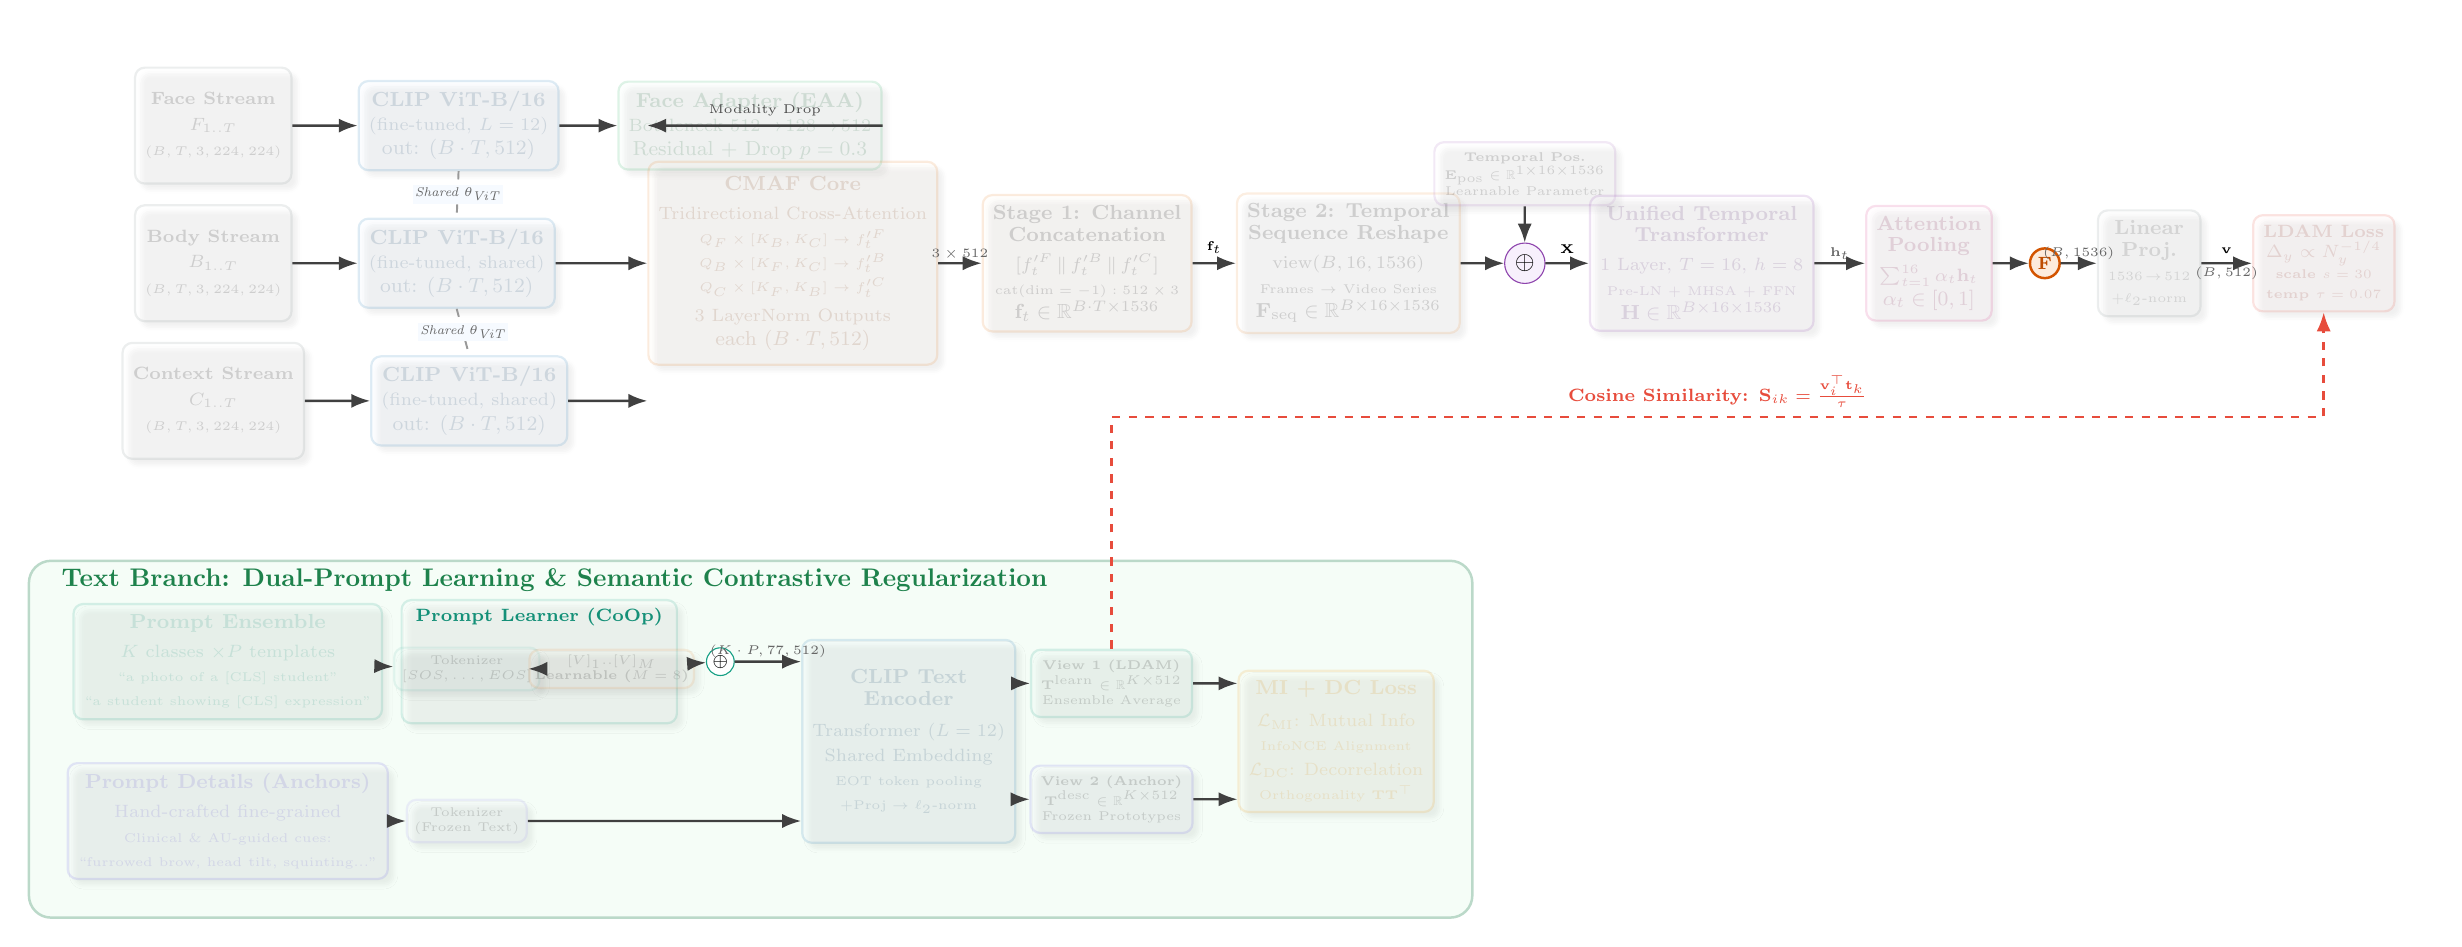
\begin{tikzpicture}[scale=0.92, transform shape, font=\footnotesize]

% ------------------------------------------------------------------------------
% 1. VISUAL BRANCH CONTAINER
% ------------------------------------------------------------------------------
\begin{scope}[local bounding box=visBranchBox]

    % Row 1: Face Stream
    \node[inputNode] (in_face) at (0, 4.4) {
        \textbf{Face Stream}\\[2pt]
        $F_{1..T}$\\[2pt]
        \tiny$(B, T, 3, 224, 224)$
    };

    \node[clipNode, right=0.9cm of in_face] (clip_face) {
        \textbf{CLIP ViT-B/16}\\
        \scriptsize (fine-tuned, $L=12$)\\
        \dimLabel{out: $(B \cdot T, 512)$}
    };

    \node[eaaNode, right=0.8cm of clip_face] (eaa) {
        \textbf{Face Adapter (EAA)}\\
        \scriptsize Bottleneck $512 \!\rightarrow\! 128 \!\rightarrow\! 512$\\
        \dimLabel{Residual + Drop $p=0.3$}
    };

    % Row 2: Body Stream
    \node[inputNode] (in_body) at (0, 2.5) {
        \textbf{Body Stream}\\[2pt]
        $B_{1..T}$\\[2pt]
        \tiny$(B, T, 3, 224, 224)$
    };

    \node[clipNode, right=0.9cm of in_body] (clip_body) {
        \textbf{CLIP ViT-B/16}\\
        \scriptsize (fine-tuned, shared)\\
        \dimLabel{out: $(B \cdot T, 512)$}
    };

    % Row 3: Context Stream
    \node[inputNode] (in_ctx) at (0, 0.6) {
        \textbf{Context Stream}\\[2pt]
        $C_{1..T}$\\[2pt]
        \tiny$(B, T, 3, 224, 224)$
    };

    \node[clipNode, right=0.9cm of in_ctx] (clip_ctx) {
        \textbf{CLIP ViT-B/16}\\
        \scriptsize (fine-tuned, shared)\\
        \dimLabel{out: $(B \cdot T, 512)$}
    };

    % Shared Weights Indicator
    \draw[sharedLine] (clip_face.south) -- node[fill=visBg, inner sep=1pt, font=\tiny\itshape, text=black!60] {Shared $\theta_{\text{ViT}}$} (clip_body.north);
    \draw[sharedLine] (clip_body.south) -- node[fill=visBg, inner sep=1pt, font=\tiny\itshape, text=black!60] {Shared $\theta_{\text{ViT}}$} (clip_ctx.north);

    % CMAF Cross-Attention Core
    \node[cmafNode] (cmaf) at (8.0, 2.5) {
        \textbf{CMAF Core}\\[2pt]
        \scriptsize Tridirectional Cross-Attention\\
        \tiny $Q_F \times [K_B, K_C] \rightarrow f_t^{\prime F}$\\
        \tiny $Q_B \times [K_F, K_C] \rightarrow f_t^{\prime B}$\\
        \tiny $Q_C \times [K_F, K_B] \rightarrow f_t^{\prime C}$\\[2pt]
        \scriptsize 3 LayerNorm Outputs\\
        \dimLabel{each $(B \cdot T, 512)$}
    };

    % Intermediate Stage 1: Channel Concatenation
    \node[baseNode, draw=cmafBorder, fill=cmafFill, right=0.6cm of cmaf, minimum width=2.0cm, minimum height=1.6cm] (cmaf_concat) {
        \textbf{Stage 1: Channel}\\[-1pt]
        \textbf{Concatenation}\\[2pt]
        \scriptsize $[f_t^{\prime F} \,\|\, f_t^{\prime B} \,\|\, f_t^{\prime C}]$\\
        \tiny $\text{cat}(\text{dim}=-1): 512 \times 3$\\
        \dimLabel{$\mathbf{f}_t \in \mathbb{R}^{B \cdot T \times 1536}$}
    };

    % Intermediate Stage 2: Temporal Sequence Reshape
    \node[baseNode, draw=cmafBorder!90, fill=white, right=0.6cm of cmaf_concat, minimum width=2.0cm, minimum height=1.6cm] (temp_reshape) {
        \textbf{Stage 2: Temporal}\\[-1pt]
        \textbf{Sequence Reshape}\\[2pt]
        \scriptsize $\text{view}(B, 16, 1536)$\\
        \tiny Frames $\rightarrow$ Video Series\\
        \dimLabel{$\mathbf{F}_{\text{seq}} \in \mathbb{R}^{B \times 16 \times 1536}$}
    };

    % Intermediate Stage 3: Temporal Positional Encoding Addition
    \node[circle, draw=tempBorder, fill=tempFill, font=\bfseries, inner sep=2pt, right=0.6cm of temp_reshape] (pos_add_master) {$\oplus$};
    \node[baseNode, draw=tempBorder!80, fill=white, above=0.5cm of pos_add_master, font=\tiny, minimum width=1.8cm] (pos_emb_master) {
        \textbf{Temporal Pos.}\\
        $\mathbf{E}_{\text{pos}} \in \mathbb{R}^{1 \times 16 \times 1536}$\\
        \tiny Learnable Parameter
    };

    % Temporal Transformer
    \node[tempNode, right=0.6cm of pos_add_master] (temporal) {
        \textbf{Unified Temporal}\\[-1pt]
        \textbf{Transformer}\\[2pt]
        \scriptsize 1 Layer, $T=16$, $h=8$\\
        \tiny Pre-LN + MHSA + FFN\\
        \dimLabel{$\mathbf{H} \in \mathbb{R}^{B \times 16 \times 1536}$}
    };

    % Attention Pooling
    \node[poolNode, right=0.7cm of temporal] (pool) {
        \textbf{Attention}\\[-1pt]
        \textbf{Pooling}\\[2pt]
        \scriptsize $\sum_{t=1}^{16} \alpha_t \mathbf{h}_t$\\
        \dimLabel{$\alpha_t \in [0, 1]$}
    };

    % Vector F
    \node[vecNode, right=0.5cm of pool] (vec_F) {$\mathbf{F}$};

    % Projection FC
    \node[projNode, right=0.5cm of vec_F] (proj) {
        \textbf{Linear}\\[-1pt]
        \textbf{Proj.}\\
        \tiny $1536 \!\rightarrow\! 512$\\[-1pt]
        \tiny $+ \ell_2\text{-norm}$
    };

    % Primary Loss: LDAM Loss
    \node[lossNode, right=0.7cm of proj] (ldam) {
        \textbf{LDAM Loss}\\
        \scriptsize $\Delta_y \propto N_y^{-1/4}$\\
        \tiny scale $s=30$\\
        \tiny temp $\tau=0.07$
    };

    % Arrows inside Visual Branch
    \draw[flowArrow] (in_face) -- (clip_face);
    \draw[flowArrow] (clip_face) -- (eaa);
    \draw[flowArrow] (eaa.east) -- node[above, font=\tiny, text=black!70] {Modality Drop} ($(cmaf.west)+(0, 1.9)$);

    \draw[flowArrow] (in_body) -- (clip_body);
    \draw[flowArrow] (clip_body) -- (cmaf.west);

    \draw[flowArrow] (in_ctx) -- (clip_ctx);
    \draw[flowArrow] (clip_ctx.east) -- ($(cmaf.west)+(0, -1.9)$);

    % Bridge Arrows
    \draw[flowArrow] (cmaf) -- node[above, dimLabel] {$3 \times 512$} (cmaf_concat);
    \draw[flowArrow] (cmaf_concat) -- node[above, font=\tiny\bfseries] {$\mathbf{f}_t$} (temp_reshape);
    \draw[flowArrow] (temp_reshape) -- (pos_add_master);
    \draw[flowArrow] (pos_emb_master) -- (pos_add_master);
    \draw[flowArrow] (pos_add_master) -- node[above, font=\tiny\bfseries] {$\mathbf{X}$} (temporal);

    \draw[flowArrow] (temporal) -- node[above, dimLabel] {$\mathbf{h}_t$} (pool);
    \draw[flowArrow] (pool) -- (vec_F);
    \draw[flowArrow] (vec_F) -- node[above, dimLabel] {$(B, 1536)$} (proj);
    \draw[flowArrow] (proj) -- node[above, font=\tiny\bfseries] {$\mathbf{v}$} node[below, dimLabel] {$(B, 512)$} (ldam);

\end{scope}

% Background for Visual Branch
\begin{scope}[on background layer]
    \node[
        fill=visBg,
        draw=visHeader!30,
        line width=0.9pt,
        rounded corners=8pt,
        fit=(visBranchBox),
        inner sep=14pt
    ] (visBgNode) {};
    \node[anchor=north west, font=\normalsize\bfseries, text=visHeader] at (visBgNode.north west) {
        \hspace{6pt} Visual Branch: Tri-Stream Spatio-Temporal Encoding \& Frame-Level Fusion
    };
\end{scope}

% ------------------------------------------------------------------------------
% 2. TEXT BRANCH CONTAINER
% ------------------------------------------------------------------------------
\begin{scope}[local bounding box=textBranchBox]

    % Row 1: Prompt Ensemble
    \node[textNode] (prompt_ens) at (0.2, -3.0) {
        \textbf{Prompt Ensemble}\\[2pt]
        \scriptsize $K$ classes $\times P$ templates\\
        \tiny ``a photo of a [CLS] student''\\
        \tiny ``a student showing [CLS] expression''
    };

    % Prompt Learner Box
    \node[baseNode, draw=promptBorder, fill=white, minimum width=3.8cm, minimum height=1.7cm] (prompt_learner) at (4.5, -3.0) {};
    \node[font=\scriptsize\bfseries, text=promptBorder!90!black, anchor=north] at (prompt_learner.north) {Prompt Learner (CoOp)};

    \node[baseNode, draw=promptBorder!60, fill=promptFill, inner sep=3pt, font=\tiny] (tok_learn) at (3.5, -3.1) {
        Tokenizer\\
        \tiny $[SOS, \dots, EOS]$
    };

    \node[baseNode, draw=cmafBorder!80, fill=cmafFill, inner sep=2pt, font=\tiny\bfseries] (learn_vec) at (5.5, -3.1) {
        $[V]_1..[V]_M$\\
        \tiny Learnable ($M=8$)
    };

    \node[circle, draw=promptBorder, fill=white, inner sep=1pt, font=\scriptsize\bfseries] (concat_sym) at (7.0, -3.0) {$\oplus$};

    % Row 2: Hand-crafted Detailed Descriptors
    \node[descNode] (prompt_desc) at (0.2, -5.2) {
        \textbf{Prompt Details (Anchors)}\\[2pt]
        \scriptsize Hand-crafted fine-grained\\
        \tiny Clinical \& AU-guided cues:\\
        \tiny ``furrowed brow, head tilt, squinting...''
    };

    \node[baseNode, draw=descBorder!60, fill=descFill, inner sep=3pt, font=\tiny] (tok_desc) at (3.5, -5.2) {
        Tokenizer\\
        \tiny (Frozen Text)
    };

    % CLIP Text Encoder
    \node[clipNode, minimum height=2.8cm, minimum width=2.4cm] (text_enc) at (9.6, -4.1) {
        \textbf{CLIP Text}\\[-1pt]
        \textbf{Encoder}\\[3pt]
        \scriptsize Transformer ($L=12$)\\
        \scriptsize Shared Embedding\\
        \tiny EOT token pooling\\
        \tiny $+ \text{Proj} \rightarrow \ell_2\text{-norm}$
    };

    % Output Embeddings
    \node[baseNode, draw=promptBorder, fill=promptFill, font=\tiny, minimum width=1.6cm] (view1_tokens) at (12.4, -3.3) {
        \textbf{View 1 (LDAM)}\\
        $\mathbf{T}^{\text{learn}} \in \mathbb{R}^{K \times 512}$\\
        \tiny Ensemble Average
    };

    \node[baseNode, draw=descBorder, fill=descFill, font=\tiny, minimum width=1.6cm] (view2_tokens) at (12.4, -4.9) {
        \textbf{View 2 (Anchor)}\\
        $\mathbf{T}^{\text{desc}} \in \mathbb{R}^{K \times 512}$\\
        \tiny Frozen Prototypes
    };

    % MI + DC Loss Module
    \node[midcNode] (midc_loss) at (15.5, -4.1) {
        \textbf{MI + DC Loss}\\[3pt]
        \scriptsize $\mathcal{L}_{\text{MI}}$: Mutual Info\\
        \tiny InfoNCE Alignment\\
        \scriptsize $\mathcal{L}_{\text{DC}}$: Decorrelation\\
        \tiny Orthogonality $\mathbf{T}\mathbf{T}^\top$
    };

    % Arrows inside Text Branch
    \draw[flowArrow] (prompt_ens) -- (tok_learn);
    \draw[flowArrow] (tok_learn) -- (learn_vec);
    \draw[flowArrow] (learn_vec) -- (concat_sym);
    \draw[flowArrow] (concat_sym) -- node[above, dimLabel] {$(K \cdot P, 77, 512)$} ($(text_enc.west)+(0, 1.1)$);

    \draw[flowArrow] (prompt_desc) -- (tok_desc);
    \draw[flowArrow] (tok_desc.east) -- ($(text_enc.west)+(0, -1.1)$);

    \draw[flowArrow] ($(text_enc.east)+(0, 0.8)$) -- (view1_tokens);
    \draw[flowArrow] ($(text_enc.east)+(0, -0.8)$) -- (view2_tokens);

    \draw[flowArrow] (view1_tokens) -- (midc_loss.west |- view1_tokens);
    \draw[flowArrow] (view2_tokens) -- (midc_loss.west |- view2_tokens);

\end{scope}

% Background for Text Branch
\begin{scope}[on background layer]
    \node[
        fill=textBg,
        draw=textHeader!30,
        line width=0.9pt,
        rounded corners=8pt,
        fit=(textBranchBox),
        inner sep=14pt
    ] (textBgNode) {};
    \node[anchor=north west, font=\normalsize\bfseries, text=textHeader] at (textBgNode.north west) {
        \hspace{6pt} Text Branch: Dual-Prompt Learning \& Semantic Contrastive Regularization
    };
\end{scope}

% ------------------------------------------------------------------------------
% 3. CROSS-BRANCH INTERACTION (COSINE SIMILARITY TO LDAM LOSS)
% ------------------------------------------------------------------------------
\draw[lossArrow] (view1_tokens.north) -- ++(0, 3.2) -| node[pos=0.25, above, font=\scriptsize\bfseries, text=lossBorder] {
    Cosine Similarity: $\mathbf{S}_{ik} = \frac{\mathbf{v}_i^\top \mathbf{t}_k}{\tau}$
} (ldam.south);

\end{tikzpicture}
\caption{\textbf{Comprehensive End-to-End Architecture of RAPT-CLIP.} The Visual Branch extracts multi-scale spatio-temporal features across Face, Body, and Context streams, enhances facial micro-expressions via the Expression-Aware Adapter (EAA), performs per-frame cross-modal contextual fusion via CMAF, and captures emotional dynamics via a Unified Temporal Transformer with Attention Pooling. The Text Branch synthesizes dual-view prompt representations optimized through LDAM, Mutual Information ($\mathcal{L}_{\text{MI}}$), and Decorrelation ($\mathcal{L}_{\text{DC}}$) losses.}
\label{fig:rapt_clip_master}
\end{figure*}

\newpage

% ==============================================================================
% DETAILED SUB-MODULE BREAKDOWNS (ZOOM-IN INSETS)
% ==============================================================================
\section*{Detailed Architectural Breakdowns of Core Sub-Modules}
To provide absolute clarity on the mathematical formulations, residual configurations, and internal routing, the subsections below detail the four foundational components of RAPT-CLIP.

\vspace{1em}

% ------------------------------------------------------------------------------
% SUBFIGURES A & B: EAA AND CMAF
% ------------------------------------------------------------------------------
\begin{figure*}[h!]
\centering
\begin{subfigure}[b]{0.44\textwidth}
\centering
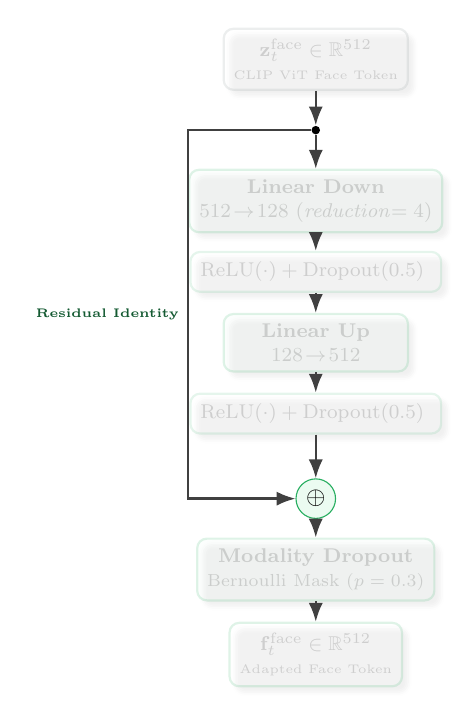
\begin{tikzpicture}[scale=0.9, transform shape, font=\footnotesize]

% Input
\node[baseNode, draw=grayBorder, fill=white, minimum width=2.4cm] (in_eaa) at (0, 6.0) {
    $\mathbf{z}_t^{\text{face}} \in \mathbb{R}^{512}$\\
    \tiny CLIP ViT Face Token
};

% Split Point for Residual
\node[circle, fill=black, inner sep=1.2pt] (split_pt) at (0, 5.0) {};

% FC Down
\node[baseNode, draw=eaaBorder, fill=eaaFill, minimum width=2.6cm] (fc_down) at (0, 4.0) {
    \textbf{Linear Down}\\
    $512 \!\rightarrow\! 128$ (\textit{reduction}$=4$)
};

% ReLU & Dropout
\node[baseNode, draw=eaaBorder!80, fill=white, minimum width=2.6cm] (act1) at (0, 3.0) {
    $\text{ReLU}(\cdot) + \text{Dropout}(0.5)$
};

% FC Up
\node[baseNode, draw=eaaBorder, fill=eaaFill, minimum width=2.6cm] (fc_up) at (0, 2.0) {
    \textbf{Linear Up}\\
    $128 \!\rightarrow\! 512$
};

% ReLU & Dropout 2
\node[baseNode, draw=eaaBorder!80, fill=white, minimum width=2.6cm] (act2) at (0, 1.0) {
    $\text{ReLU}(\cdot) + \text{Dropout}(0.5)$
};

% Add Node
\node[circle, draw=eaaBorder, fill=eaaFill, font=\bfseries, inner sep=2pt] (add_node) at (0, -0.2) {$\oplus$};

% Modality Dropout
\node[baseNode, draw=eaaBorder, fill=eaaFill, minimum width=2.6cm] (mod_drop) at (0, -1.2) {
    \textbf{Modality Dropout}\\
    \scriptsize Bernoulli Mask ($p=0.3$)
};

% Output
\node[baseNode, draw=eaaBorder, fill=white, minimum width=2.4cm] (out_eaa) at (0, -2.4) {
    $\mathbf{f}_t^{\text{face}} \in \mathbb{R}^{512}$\\
    \tiny Adapted Face Token
};

% Flow Arrows
\draw[flowArrow] (in_eaa) -- (split_pt);
\draw[flowArrow] (split_pt) -- (fc_down);
\draw[flowArrow] (fc_down) -- (act1);
\draw[flowArrow] (act1) -- (fc_up);
\draw[flowArrow] (fc_up) -- (act2);
\draw[flowArrow] (act2) -- (add_node);
\draw[flowArrow] (add_node) -- (mod_drop);
\draw[flowArrow] (mod_drop) -- (out_eaa);

% Residual Skip Connection
\draw[flowArrow] (split_pt) -- ++(-1.8, 0) |- node[pos=0.25, left, font=\tiny\bfseries, text=eaaText] {Residual Identity} (add_node);

\end{tikzpicture}
\caption{\textbf{Expression-Aware Adapter (EAA)}. A bottleneck architecture adapting frozen visual tokens to subtle classroom expressions while preserving foundational CLIP weights.}
\label{fig:eaa_detail}
\end{subfigure}
\hfill
\begin{subfigure}[b]{0.54\textwidth}
\centering
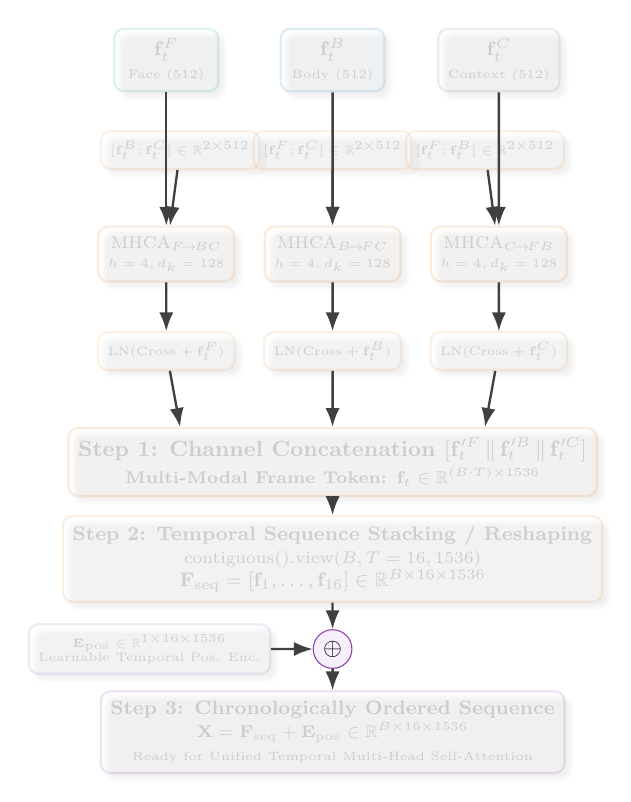
\begin{tikzpicture}[scale=0.88, transform shape, font=\footnotesize]

% 3 Inputs
\node[baseNode, draw=eaaBorder, fill=eaaFill, minimum width=1.5cm] (in_f) at (0, 5.8) {$\mathbf{f}_t^F$\\ \tiny Face ($512$)};
\node[baseNode, draw=clipBorder, fill=clipFill, minimum width=1.5cm] (in_b) at (2.4, 5.8) {$\mathbf{f}_t^B$\\ \tiny Body ($512$)};
\node[baseNode, draw=grayBorder, fill=grayFill, minimum width=1.5cm] (in_c) at (4.8, 5.8) {$\mathbf{f}_t^C$\\ \tiny Context ($512$)};

% KV Concat Boxes
\node[baseNode, draw=cmafBorder!80, fill=white, font=\tiny] (kv_bc) at (0.2, 4.5) {$[\mathbf{f}_t^B; \mathbf{f}_t^C] \in \mathbb{R}^{2 \times 512}$};
\node[baseNode, draw=cmafBorder!80, fill=white, font=\tiny] (kv_fc) at (2.4, 4.5) {$[\mathbf{f}_t^F; \mathbf{f}_t^C] \in \mathbb{R}^{2 \times 512}$};
\node[baseNode, draw=cmafBorder!80, fill=white, font=\tiny] (kv_fb) at (4.6, 4.5) {$[\mathbf{f}_t^F; \mathbf{f}_t^B] \in \mathbb{R}^{2 \times 512}$};

% 3 Multi-Head Attention Blocks
\node[baseNode, draw=cmafBorder, fill=cmafFill, minimum width=1.8cm, font=\scriptsize] (mha_f) at (0, 3.0) {
    $\text{MHCA}_{F \!\rightarrow\! BC}$\\
    \tiny $h=4, d_k=128$
};

\node[baseNode, draw=cmafBorder, fill=cmafFill, minimum width=1.8cm, font=\scriptsize] (mha_b) at (2.4, 3.0) {
    $\text{MHCA}_{B \!\rightarrow\! FC}$\\
    \tiny $h=4, d_k=128$
};

\node[baseNode, draw=cmafBorder, fill=cmafFill, minimum width=1.8cm, font=\scriptsize] (mha_c) at (4.8, 3.0) {
    $\text{MHCA}_{C \!\rightarrow\! FB}$\\
    \tiny $h=4, d_k=128$
};

% Residual & Norm
\node[baseNode, draw=cmafBorder!80, fill=white, font=\tiny] (ln_f) at (0, 1.6) {$\text{LN}(\text{Cross} + \mathbf{f}_t^F)$};
\node[baseNode, draw=cmafBorder!80, fill=white, font=\tiny] (ln_b) at (2.4, 1.6) {$\text{LN}(\text{Cross} + \mathbf{f}_t^B)$};
\node[baseNode, draw=cmafBorder!80, fill=white, font=\tiny] (ln_c) at (4.8, 1.6) {$\text{LN}(\text{Cross} + \mathbf{f}_t^C)$};

% Concatenation
\node[baseNode, draw=cmafBorder, fill=cmafFill, minimum width=4.8cm, font=\small\bfseries] (concat_cmaf) at (2.4, 0.0) {
    Step 1: Channel Concatenation $[\mathbf{f}_t^{\prime F} \,\|\, \mathbf{f}_t^{\prime B} \,\|\, \mathbf{f}_t^{\prime C}]$\\
    \scriptsize Multi-Modal Frame Token: $\mathbf{f}_t \in \mathbb{R}^{(B \cdot T) \times 1536}$
};

% Temporal Stacking
\node[baseNode, draw=cmafBorder!90, fill=white, minimum width=4.8cm] (seq_stack) at (2.4, -1.4) {
    \textbf{Step 2: Temporal Sequence Stacking / Reshaping}\\
    \scriptsize $\text{contiguous}().\text{view}(B, T=16, 1536)$\\
    \dimLabel{$\mathbf{F}_{\text{seq}} = [\mathbf{f}_1, \dots, \mathbf{f}_{16}] \in \mathbb{R}^{B \times 16 \times 1536}$}
};

% Positional Embedding Addition
\node[circle, draw=tempBorder, fill=tempFill, font=\bfseries, inner sep=2pt] (pos_add_sub) at (2.4, -2.7) {$\oplus$};
\node[baseNode, draw=tempBorder!80, fill=white, left=0.6cm of pos_add_sub, font=\tiny] (pos_emb_sub) {
    $\mathbf{E}_{\text{pos}} \in \mathbb{R}^{1 \times 16 \times 1536}$\\
    \tiny Learnable Temporal Pos. Enc.
};

% Output to Temporal Transformer
\node[baseNode, draw=tempBorder, fill=tempFill, minimum width=4.8cm] (bridge_out) at (2.4, -3.9) {
    \textbf{Step 3: Chronologically Ordered Sequence}\\
    \scriptsize $\mathbf{X} = \mathbf{F}_{\text{seq}} + \mathbf{E}_{\text{pos}} \in \mathbb{R}^{B \times 16 \times 1536}$\\
    \tiny Ready for Unified Temporal Multi-Head Self-Attention
};

% Connecting Arrows
\draw[flowArrow] (in_f) -- (mha_f);
\draw[flowArrow] (in_b) -- (mha_b);
\draw[flowArrow] (in_c) -- (mha_c);

\draw[flowArrow] (kv_bc) -- (mha_f);
\draw[flowArrow] (kv_fc) -- (mha_b);
\draw[flowArrow] (kv_fb) -- (mha_c);

\draw[flowArrow] (mha_f) -- (ln_f);
\draw[flowArrow] (mha_b) -- (ln_b);
\draw[flowArrow] (mha_c) -- (ln_c);

\draw[flowArrow] (ln_f) -- ($(concat_cmaf.north)+(-2.2, 0)$);
\draw[flowArrow] (ln_b) -- (concat_cmaf.north);
\draw[flowArrow] (ln_c) -- ($(concat_cmaf.north)+(2.2, 0)$);

\draw[flowArrow] (concat_cmaf) -- (seq_stack);
\draw[flowArrow] (seq_stack) -- (pos_add_sub);
\draw[flowArrow] (pos_emb_sub) -- (pos_add_sub);
\draw[flowArrow] (pos_add_sub) -- (bridge_out);

\end{tikzpicture}
\caption{\textbf{CMAF-to-Temporal Bridging Flow}. Tridirectional cross-attention routes mutual spatial context, followed by channel concatenation, 16-frame temporal sequence reshaping, and chronological positional encoding injection.}
\label{fig:cmaf_detail}
\end{subfigure}
\end{figure*}

\vspace{1.5em}

% ------------------------------------------------------------------------------
% SUBFIGURES C & D: TEMPORAL + ATTENTION POOLING AND TEXT BRANCH / LOSSES
% ------------------------------------------------------------------------------
\begin{figure*}[h!]
\centering
\begin{subfigure}[b]{0.48\textwidth}
\centering
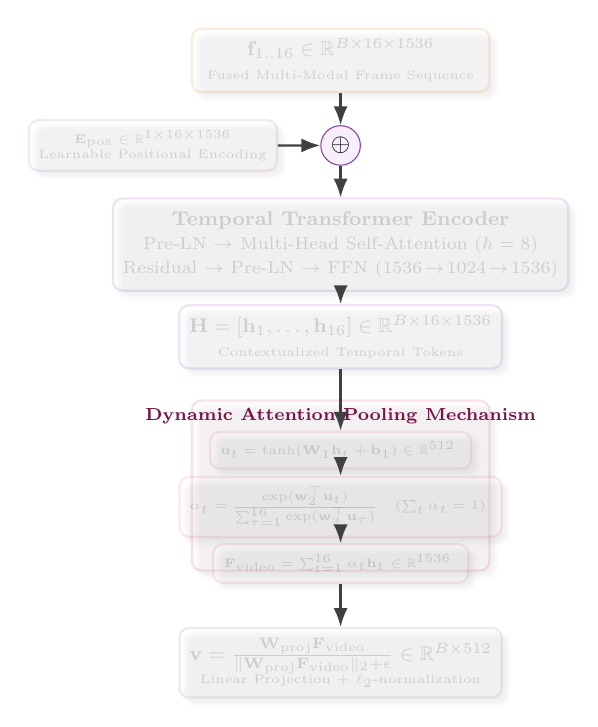
\begin{tikzpicture}[scale=0.9, transform shape, font=\footnotesize]

% Input Sequence
\node[baseNode, draw=cmafBorder, fill=white, minimum width=4.2cm] (temp_in) at (0, 7.0) {
    $\mathbf{f}_{1..16} \in \mathbb{R}^{B \times 16 \times 1536}$\\
    \tiny Fused Multi-Modal Frame Sequence
};

% Positional Embedding Add
\node[circle, draw=tempBorder, fill=tempFill, font=\bfseries, inner sep=2pt] (pos_add) at (0, 5.8) {$\oplus$};
\node[baseNode, draw=tempBorder!80, fill=white, left=0.6cm of pos_add, font=\tiny] (pos_emb) {
    $\mathbf{E}_{\text{pos}} \in \mathbb{R}^{1 \times 16 \times 1536}$\\
    \tiny Learnable Positional Encoding
};

% Transformer Layer
\node[baseNode, draw=tempBorder, fill=tempFill, minimum width=4.2cm, minimum height=1.3cm] (tx_layer) at (0, 4.4) {
    \textbf{Temporal Transformer Encoder}\\
    \scriptsize Pre-LN $\rightarrow$ Multi-Head Self-Attention ($h=8$)\\
    \scriptsize Residual $\rightarrow$ Pre-LN $\rightarrow$ FFN ($1536 \!\rightarrow\! 1024 \!\rightarrow\! 1536$)
};

% Temporal Features H
\node[baseNode, draw=tempBorder, fill=white, minimum width=3.8cm] (feat_H) at (0, 3.1) {
    $\mathbf{H} = [\mathbf{h}_1, \dots, \mathbf{h}_{16}] \in \mathbb{R}^{B \times 16 \times 1536}$\\
    \tiny Contextualized Temporal Tokens
};

% Attention Pooling Inner Block
\node[baseNode, draw=poolBorder, fill=poolFill, minimum width=4.2cm, minimum height=2.4cm] (pool_box) at (0, 1.0) {};
\node[font=\scriptsize\bfseries, text=poolText, anchor=north] at (pool_box.north) {Dynamic Attention Pooling Mechanism};

\node[baseNode, draw=poolBorder!80, fill=white, font=\tiny, minimum width=3.6cm] (score_net) at (0, 1.5) {
    $\mathbf{u}_t = \tanh(\mathbf{W}_1 \mathbf{h}_t + \mathbf{b}_1) \in \mathbb{R}^{512}$
};

\node[baseNode, draw=poolBorder!80, fill=white, font=\tiny, minimum width=3.6cm] (softmax_pool) at (0, 0.7) {
    $\alpha_t = \frac{\exp(\mathbf{w}_2^\top \mathbf{u}_t)}{\sum_{\tau=1}^{16} \exp(\mathbf{w}_2^\top \mathbf{u}_\tau)} \quad (\sum_t \alpha_t = 1)$
};

\node[baseNode, draw=poolBorder!80, fill=white, font=\tiny, minimum width=3.6cm] (weighted_sum) at (0, -0.1) {
    $\mathbf{F}_{\text{video}} = \sum_{t=1}^{16} \alpha_t \mathbf{h}_t \in \mathbb{R}^{1536}$
};

% Output
\node[baseNode, draw=grayBorder, fill=grayFill, minimum width=4.0cm] (proj_out) at (0, -1.5) {
    $\mathbf{v} = \frac{\mathbf{W}_{\text{proj}}\mathbf{F}_{\text{video}}}{\|\mathbf{W}_{\text{proj}}\mathbf{F}_{\text{video}}\|_2 + \epsilon} \in \mathbb{R}^{B \times 512}$\\
    \tiny Linear Projection + $\ell_2$-normalization
};

% Arrows
\draw[flowArrow] (temp_in) -- (pos_add);
\draw[flowArrow] (pos_emb) -- (pos_add);
\draw[flowArrow] (pos_add) -- (tx_layer);
\draw[flowArrow] (tx_layer) -- (feat_H);
\draw[flowArrow] (feat_H) -- (score_net);
\draw[flowArrow] (score_net) -- (softmax_pool);
\draw[flowArrow] (softmax_pool) -- (weighted_sum);
\draw[flowArrow] (weighted_sum) -- (proj_out);

\end{tikzpicture}
\caption{\textbf{Temporal Transformer \& Attention Pooling}. Models dynamic long-range frame transitions and adaptively weights emotionally prominent segments.}
\label{fig:temporal_detail}
\end{subfigure}
\hfill
\begin{subfigure}[b]{0.48\textwidth}
\centering
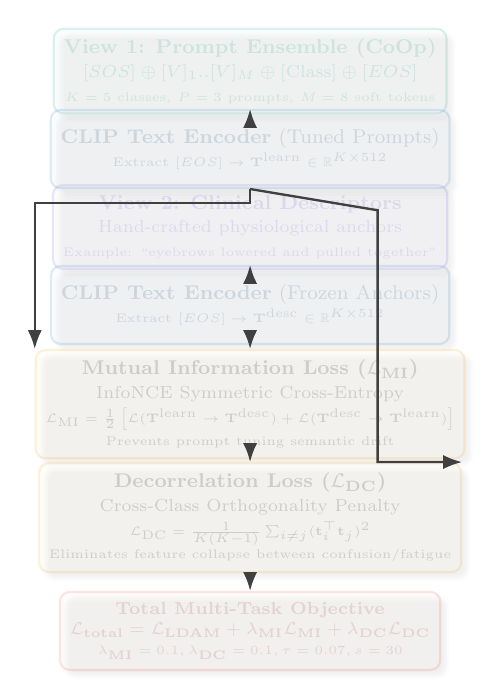
\begin{tikzpicture}[scale=0.9, transform shape, font=\footnotesize]

% Prompts Top: View 1
\node[textNode, minimum width=3.8cm] (view1_in) at (0, 7.0) {
    \textbf{View 1: Prompt Ensemble (CoOp)}\\
    \scriptsize $[SOS] \oplus [V]_1..[V]_M \oplus [\text{Class}] \oplus [EOS]$\\
    \tiny $K=5$ classes, $P=3$ prompts, $M=8$ soft tokens
};

% Prompts Bottom: View 2
\node[descNode, minimum width=3.8cm] (view2_in) at (0, 4.8) {
    \textbf{View 2: Clinical Descriptors}\\
    \scriptsize Hand-crafted physiological anchors\\
    \tiny Example: ``eyebrows lowered and pulled together''
};

% Text Encoders
\node[clipNode, minimum width=3.8cm] (text_enc_view1) at (0, 5.9) {
    \textbf{CLIP Text Encoder} (Tuned Prompts)\\
    \tiny Extract $[EOS] \rightarrow \mathbf{T}^{\text{learn}} \in \mathbb{R}^{K \times 512}$
};

\node[clipNode, minimum width=3.8cm] (text_enc_view2) at (0, 3.7) {
    \textbf{CLIP Text Encoder} (Frozen Anchors)\\
    \tiny Extract $[EOS] \rightarrow \mathbf{T}^{\text{desc}} \in \mathbb{R}^{K \times 512}$
};

% MI Loss Block
\node[baseNode, draw=midcBorder, fill=midcFill, minimum width=4.2cm] (mi_box) at (0, 2.3) {
    \textbf{Mutual Information Loss ($\mathcal{L}_{\text{MI}}$)}\\
    \scriptsize InfoNCE Symmetric Cross-Entropy\\
    \tiny $\mathcal{L}_{\text{MI}} = \frac{1}{2}\left[\mathcal{L}(\mathbf{T}^{\text{learn}} \rightarrow \mathbf{T}^{\text{desc}}) + \mathcal{L}(\mathbf{T}^{\text{desc}} \rightarrow \mathbf{T}^{\text{learn}})\right]$\\
    \tiny Prevents prompt tuning semantic drift
};

% DC Loss Block
\node[baseNode, draw=midcBorder, fill=midcFill, minimum width=4.2cm] (dc_box) at (0, 0.7) {
    \textbf{Decorrelation Loss ($\mathcal{L}_{\text{DC}}$)}\\
    \scriptsize Cross-Class Orthogonality Penalty\\
    \tiny $\mathcal{L}_{\text{DC}} = \frac{1}{K(K-1)} \sum_{i \ne j} (\mathbf{t}_i^{\top} \mathbf{t}_j)^2$\\
    \tiny Eliminates feature collapse between confusion/fatigue
};

% Joint Loss
\node[lossNode, minimum width=4.2cm] (joint_loss) at (0, -0.9) {
    \textbf{Total Multi-Task Objective}\\
    $\mathcal{L}_{\text{total}} = \mathcal{L}_{\text{LDAM}} + \lambda_{\text{MI}}\mathcal{L}_{\text{MI}} + \lambda_{\text{DC}}\mathcal{L}_{\text{DC}}$\\
    \tiny $\lambda_{\text{MI}}=0.1, \lambda_{\text{DC}}=0.1, \tau=0.07, s=30$
};

% Arrows
\draw[flowArrow] (view1_in) -- (text_enc_view1);
\draw[flowArrow] (view2_in) -- (text_enc_view2);

\draw[flowArrow] (text_enc_view1.south) -- ++(0, -0.2) -| (mi_box.north west);
\draw[flowArrow] (text_enc_view2.south) -- (mi_box.north);

\draw[flowArrow] (text_enc_view1.south) -- ++(1.8, -0.3) |- (dc_box.north east);

\draw[flowArrow] (mi_box) -- (dc_box);
\draw[flowArrow] (dc_box) -- (joint_loss);

\end{tikzpicture}
\caption{\textbf{Dual-Prompt Architecture \& Contrastive Losses}. View 1 learns task-adaptive representations while View 2 enforces semantic grounding and cross-class orthogonality.}
\label{fig:loss_detail}
\end{subfigure}
\end{figure*}

\end{document}
